%% Computer Networks Project Report Latex file.
%% Completed By Yuyang Rong(rongyy@shanghaitech.edu.cn) and 
%% Jianxiong Cai(caijx@shanghaitech.edu.cn)
%%
%% To edit this file, please use indentions with tab size of 2.
%%

\documentclass[conference,compsoc]{IEEEtran}
\usepackage{cite}
\usepackage{listings}
\usepackage{mathtools}
\usepackage{amsmath,amsthm,amssymb,amsfonts}
\usepackage{array}
\usepackage{tikz}
\usetikzlibrary{automata,positioning}
\lstset{
	basicstyle=\small\ttfamily,
	columns=fullflexible,
	tabsize=1
}
\begin{document}
\title{
	Computer Networks Course Report
}
% author names and affiliations
% use a multiple column layout for up to three different
% affiliations
\author{
	\IEEEauthorblockN{Yuyang Rong}
	\IEEEauthorblockA{
		School of Information Science and Technology \\
		ShanghaiTech University \\
		Student ID: 69850764 \\
	}
\and
	\IEEEauthorblockN{Jianxiong Cai}
	\IEEEauthorblockA{
		School of Information Science and Technology \\
		ShanghaiTech University \\
		Student ID: 67771603 \\
	}
}

\maketitle

% As a general rule, do not put math, special symbols or citations
% in the abstract
\begin{abstract}
A quick brown fox jumps over a lazy dog.
\end{abstract}

%%%%%%%%%%%%%%%%%%%%%%%%%%%%%%%%%%%%%%%%%%%%%%%%%%%%%%%%%%%%%%%%%%%%%
%%
%% Project 1: physical layer
%%
%%%%%%%%%%%%%%%%%%%%%%%%%%%%%%%%%%%%%%%%%%%%%%%%%%%%%%%%%%%%%%%%%%%%%
\section{Project 1: physical layer}
	
	%TOCHECK
	\subsection{Sound card and DataLine}
		Java provides access to sound card and uses an abstract call data line. 
		Difficult as it may to try to use this, we have finally finished this project and I can hardly remember how to use it:).
		\par
		However, there are problems we discovered and solved in terms of sound card.
		One particular problem is that the sound card will keep replaying the content in the buffer if no new data is offered.
		In project 2, we kept receiving the same ACK packet is caused by this feature.
		To tackle with this problem, we choose to start the device only when we are transmitting something and shutdown it down once the transmission is done.
		However, the downside of this solution is that accessing IO device has low priority in OS and thus takes long time. 
		Such acquiring and releasing took 0.5 more second when sending 10,000 bits to the other side.

	%TOCHECK
	\subsection{Data Definition}
		We defined the frame as shown in table \ref{PhyLayer_dataDef}.
		\begin{table}[ht]
		\begin{center}\begin{tabular}{m{1cm}m{1cm}m{1cm}m{1cm}}\label{PhyLayer_dataDef}
		Offset                        & 0                        & 8                        & 12                        \\ \hline
		\multicolumn{1}{|l|}{Content} & \multicolumn{1}{l|}{len} & \multicolumn{1}{l|}{crc8} & \multicolumn{1}{l|}{data} \\ \hline
		\end{tabular}\end{center}
		\caption{The Definition of a Physical packet}
		\end{table}
		\par
		The first byte is used to indicate how long is the data part. 
		This feature is not added until project 2. 
		Using one byte to indicate length, we have a maximum length of physical packet of 256 bytes.
		It is worth noticing that the CRC8 will not include the first byte, but the data byte.
		The intuition is that if the length get wrong, the CRC check will still not pass.

	%TOCHECK
	\subsection{Modulation \& Demodulation}
		\subsubsection{Preamble} 
			Before we can talk about modulation, we have to determine when the signal starts. We added a preamble to every packet and it's a signature sin wave defined below:
			\begin{equation*}\begin{aligned}
				& d_k = sin(2\pi\omega_k) \\
				& \omega_k = \omega_{k-1} + \frac{f_k + f_{k-1}}{2\times sr} \\
				& f_k = h - |k-\frac{1}{2}n|\frac{h-l}{n} \\
				s.t. \\
				& \omega_0 = 0 \\
				& sr = 48,000 \text{(Samples/s)}\\
				& h = 10,000 \text{(Hz), } l = 2,000 \text{(Hz)}
			\end{aligned}\end{equation*}
			\par
			Such preamble will have a nice feature that the dot product is very small unless it's perfectly aligned. 
			In practice, the alignment error will only shift by one or two samples.
		\subsection{Modulation \& Demodulation}
			We adopted PSK, where bit 0 and 1 corresponds to $cos(2\pi f)$ and $cos(2\pi f + \pi)$. 
			But in reality it's easier to modulate as we has calculated $cos(2\pi f)$ in advance and we can multiply it by $-1$ and get $cos(2\pi f)$.
			Thus the calculation of triangular functions is limited.
			When demodulating, we take the bit and multiply it with $cos(2\pi f)$ we can get $1$ and $-1$ corresponding to 1 and 0.
			\begin{equation*}\begin{aligned}
				& cos(2\pi f)cos(2\pi f) = \frac{1}{2}(cos(4\pi f) - 1) \\
				& \int_0^\frac{1}{2f} cos(4\pi ft)dt \approx \sum_{k=1}^{24}cos(4\pi fk)\frac{k}{sr} = 0
			\end{aligned}\end{equation*}
			\par
			In practice, we cannot use arbitrarily long samples to represent a bit. We used only 24 samples. 
			24 samples per bit allows us a bandwidth of 2kbps if we have 48,000 sample rate and don't consider preambles.
			\par
			We could have adopted QPSK and our bandwidth can boost to two times what we have now. 
			However, we have to calculate more triangular functions. 
			What's worse, when demodulating, we cannot distinguish $-1$ and $-0.5$ very well, leading higher risk of transfer failure.
			This problem, however, can be tackled if we considered frequency shift caused by hardware and calibrate our software parameters automatically.

	%TOCHECK
	\subsection{Frequency Shift}
		At first attempts to create physical layer, we realized that although the command we issued was to make a sound of 10kHz, what we really got tend to have a 10Hz frequency shift.
		We thought it is not a problem at first, but as the project went on, especially when we are dealing with FDM, this become more problematic.
		We were suggested by Pang Anqi that there is a way to correct the frequency using software, but we never had time to finish that.

	%TOCHECK
	\subsection{FDM}
		Although we are given the option to implement OFDM, the involvement of FFT and all other Signal and System stuff was way too difficult for two poor student. 
		So we adopted, or reinvented(true story, we were thinking how to improve the usage of each channel), FDM.
		FDM is based on one simple formula:
		\begin{equation*} \begin{aligned}
			& \int_{0}^{\frac{1}{2}T} cos(t)cos(kt)dt = 0 \\
			s.t. \\
			& k \in \mathbb{N}
		\end{aligned} \end{equation*}
		This formula implies that we can transmit data in 8 channels simultaneously, the demodulation process of one particular channel will not be interfered by the presence of other 7 channels as their signal will be canceled by the $cos$ function we applied.
	
	%TOCHECK
	\subsection{Frequency Response and Channel picking}
		We have to face the fact that the frequency response of the sound care is not a perfectly line, but a curved line where the amplititude will drop by almost a half as the frequency goes up to 10kHz.
		We didn't realize this when we are not using FDM. 
		At the first stages of FDM, we used frequency from 8kHz to 15kHz where the last few bits of a byte always go wrong. 
		That's when we realized that the frequency response can be a problem.
		Finally, after trials and errors, we picked 1kHz to 8kHz.
		\par
		We tried to add more channels without going over 10kHz, however, the minimum bandwidth we found is 700Hz, which made it impossible to have 16 channels without touching 10kHz.

	%TOCHECK
	\subsection{Java experience: OOP}
		This course is challenging as this is our first time to write Java code.
		Before this, all we know about Java is it's spelling and it's a horrible language(so what? C is also a horrible language :) ).
		As this project goes on, we also learned a lot about Java and it's design philosophy.
		\par
		The first philosophy we experienced is OOP. 
		Everything is an \lstinline{Object} is a great idea.
		Although Python 3(Have to specifically point out 3 not 2, as there are classes in Python 2 that is not inherited from \lstinline{Object})
		In this project, we not only experienced how convenient the abstract provided by the built in class like \lstinline{DataLine} is, but we also created a few classes ourselves.
		We realized that this enforcement can force programmers to program neatly and the code is automatically readable.
		\par
		However, we have to point out that the names in Java is so long that many lines involving multiple variables and classes have to be split in to two or more lines.
		\par
		OOP also has a powerful tool call inheritance(in Java, it's called extend), it's a shame we didn't use this feature in this 4 projects. 
		Another feature we touched a little is \lstinline{implements}.
		We used it when a class has two threads then we have to implement \lstinline{Run}.

%%%%%%%%%%%%%%%%%%%%%%%%%%%%%%%%%%%%%%%%%%%%%%%%%%%%%%%%%%%%%%%%%%%%%
%%
%% Project 2: mac layer
%%
%%%%%%%%%%%%%%%%%%%%%%%%%%%%%%%%%%%%%%%%%%%%%%%%%%%%%%%%%%%%%%%%%%%%%
\section{Project 2: mac layer}
	
	%TOCHECK
	\subsection{Mac Packet}
		The basic unit in mac layer is a new type of packet called \lstinline{MacPacket}. 
		It contains all the data, the type of this packet, it's current status and the time it's been sent. 
		The Mac address of the sender and the received will also be stored.
		\subsubsection{Conversion between byte array and MacPacket}
			We have to examine the definition of the byte array first. It is show in the table \ref{MacPacket_dataDef}
			\begin{table}[ht]
			\begin{center}\begin{tabular}{m{0.5cm}m{2cm}m{0.5cm}m{0.5cm}m{1cm}m{1cm}}\label{MacPacket_dataDef}
				Offset                        & 0                       & 8                        & 10                       & 12                        & 16                        \\ \hline
				\multicolumn{1}{|l|}{Content} & \multicolumn{1}{l|}{ID} & \multicolumn{1}{l|}{src} & \multicolumn{1}{l|}{dst} & \multicolumn{1}{l|}{type} & \multicolumn{1}{l|}{data} \\ \hline
			\end{tabular}\end{center}
			\caption{The definition of a MacPacket}
			\end{table}
			\par
			To convert a MacPacket to byte array is somewhat simple, just use \lstinline{System.arraycopy(...)} is good. But to convert a byte array to \lstinline{MacPacket}, we need to carefully take the bits out by using shift.

	\subsection{Request}
		We can not allow packet to be send directly. To send a packet, the user has to call \lstinline{MacLayer.requestSend(...)} and then the mac layer can begin to process. 
		As a matter of fact, user can not call \lstinline{MacLayer.send()} directly as it's a private function.
		\par
		The parameters in the function above varies. We provided a lot of interface so that it is handy in use. You can use an instance of \lstinline{MacPacket} to request send. 
		\begin{lstlisting}[linewidth=\columnwidth,language=Java]
			MacLayer.requestSend(MacPacket);
		\end{lstlisting}
		\par
		Other methods to request a send service is to give a raw byte array if it is a data packet or just state the length of the incoming data if it is a control packet at the head of every data stream.
		\begin{lstlisting}[linewidth=\columnwidth,language=Java]
			MacLayer.requestSend(byte[] raw_data);
			MacLayer.requestSend(int data_len);
		\end{lstlisting}
		In these two function, we will pack the data into a \lstinline{MacPacket} and call \lstinline{MacLayer.requestSend(MacPacket)}
		\par
		Once a packet is requested to be sent, first thing we do in \lstinline{MacLayer.requestSend(MacPacket)} is assign this packet an id. 
		Packet ID is the identifier to guarantee that we don't receive the same packet.
		(This is possible when the ACK we replied is lost.)
		With id setup, we will put the packet in the waiting queue. We will determine whether it's a priority one(mainly ACK packet, we added another priority packet MACPING in project 3) or not. 
		Priority packet will be placed at the head of the waiting queue so that it can be sent first, other packets will be placed at the tail of the queue and follow FIFO. 
		\par
		We may have a design flaw here. 
		The fact that we reply ACK first may lead to normal data being chocked if we are receiving enormous packets and busy replying ACKs.
	\subsection{Send}
		\lstinline{MacLayer.send()} is a loop that only stops upon user's call.
		In each iteration, it will take the a window of the waiting queue. 
		For each packet in the window, our action depends on the label of the packet.
		\par
		If the label is \lstinline{MacPacket.STATUS_WAITING}, it will be converted to raw \lstinline{byte[]} and send it by calling \lstinline{Transmitter.transmitOnePack(byte[] data)}. 
		The status of the packet will be labeled \lstinline{MacPacket.STATUS_ACKED} if this packet need no ACK(for example, ACK packet need no ACK, or it would be infinity of ACKs wondering in the channel busying ACK each other.). 
		Packets that needs to be ACKed will be labeled \lstinline{MacPacket.STATUS_SENT}.
		\par 
		If the label is \lstinline{MacPacket.STATUS_SENT}. 
		We will examine the time stamp in the packet and compare with the current to determine if the packet has time out. Upon timeout, we change the label to \lstinline{MacPacket.STATUS_WAITING} so that it can be resent. 
		We will also add the counter inside the packet so that we know how many time it has been resent. 
		If we have resend it too much, we will report a link error.
		\par
		When one window's packet have been processed, we will run a second pass on that window and re-examine the labels. 
		This time we are looking for \lstinline{MacPacket.STATUS_ACKED}. 
		We moves the window foreword if the head of the waiting queue has been ACKed. 
		Also, we will take back the id of that ACKed packet so that late comers can re-use the id.

	%TOCHECK
	\subsubsection{Receive}
		\lstinline{MacLayer.receive()} is also a function that loops until the user stops it.
		\par
		At each iteration, it will try to receive a frame by calling \lstinline{Receiver.receiveOnePack()}.
		The function may fail as there is nothing to be received and return an empty array, then the iteration ends and goes to next iteration.
		Correct frame can be received, then we will transform the received \lstinline{byte[]} to \lstinline{MacPacket} without certain informations like time stamp, but that will not hurt.
		With an instance of \lstinline{MacPacket} we will check the mac address of the packet. 
		If the address is not correct, we will start the next iteration. 
		We will send an ACK if this is a data packet and put it into data buffer. 
		If the packet is and ACK packet, we will check the find the packet that is being ACKed and change it's label to \lstinline{MacPacket.STATUS_ACKED}.
		A patch we added for MACPING is to either reply that MACPING or calculate the time eclipsed.

	%TOCHECK
	\subsection{Thread pool}\label{Thread pool}
		\lstinline{MacLayer.send()} and \lstinline{MacLayer.receive()} should be in two threads. 
		We set up a starter and a stopper to help user better handle these two threads at the same time.
		The user has to call \lstinline{MacLayer.startMacLayer()} to start them and use \lstinline{MacLayer.stopMacLayer} to stop the threads.
	
	%TOCHECK
	\subsection{Sequential arriving data}
		To transmit large file, we should use more packets and then assembly them after transmission. 
		This is when sequential arrival become crucial. If the sequence of the data cannot be guaranteed, then we cannot correctly assemble the data.
		\par  
		Using ID to assemble the data may not be useful since the id can be broken and out of order because ACK packet and MACPING packet also takes id.
		The solution we propose is to add a receiving window in \lstinline{MacLayer.receive()}. 
		We store all the packet in a buffer that is invisible to the user(private buffer). 
		Only when the data in the private buffer are in order do we transfer them to the public buffer for the user to take.
		\par
		However, in real, we didn't have a private buffer, but a private array using id to do the indexing. 
		The public buffer, however, we used \lstinline{java.util.concurrent.ArrayBlockingQueue}.
		This is a thread safe data structure where the taker will be preempted if the queue is empty since the taker is (probably) in the main thread the giver is always in the receive thread.
		\par
		Sadly, this design only worked in project 2 and 3. 
		In project 3 we realized that this is a flawed design. 
		If fails when the MacLayer is both sending and receiving. 
		Then the window will be chocked by ACKs and the private buffer can never transfer anything to public buffer. 
		In project 4, we removed this design.
	
	%TOCHECK
	\subsection{Signal Detection}
		Whenever sending a frame, the sender must make sure that the channel is clean and is good for transmission.
		The process is somewhat similar to CSMA/CD, yet there is no detecting while sending.
		\par
		The sending process will start only when the moving average power of the channel is low enough. The avg power should satisfy:
		\begin{equation}\begin{aligned}
		avg_k \\
		& = 
			\frac{win\_size-1}{win\_size}avg_{k-1} + 
			\frac{1}{win\_size} * power_k \\
		& > thr
		\end{aligned}\end{equation}
		where in our implementation, we have:
		\begin{equation*}\begin{aligned} 
			& win\_size = 24 \\
			& thr = 0.3 
		\end{aligned}\end{equation*}
		\par
		If the power is	greater than the threshold we set, we will wait sometime, by default we wait 10ms.
		\par 
		We didn't add collection detection in out implementation due to one design flaw. 
		We split the physical layer to two independent part: sender and receiver. 
		The fact that these two components cannot communicate leads to the hardship when writing collection detection. 
		We hold one assumption while doing this project, that once the transmission is started, no one will interrupted because other senders should be listening the channel and hold off sending only when the average power goes down.
	%TOCHECK
	\subsection{Java experience: reference}
		\subsubsection{Bit Shift} 
			While we are converting byte array to \lstinline{MacPacket}, we were astonished to find that add and minus(+ / -) generally has more priority than shift(<< / >>).
		\subsubsection{Reference} 
			In Java, everything is a reference. 
			We took the fall at the first time by accidentally change the value of a reference as we thought we are dealing with a new instance. 
			However, once we realized this, we utilized this in project 3. 
			In project 3, we have a waiting queue with 3 threads.
			Using reference allows us to access the same instance across 3 threads with no problem.
			Furthermore, in project 3 \& 4, when we have more instances of \lstinline{MacLayer}, reference allows us to only create one \lstinline{MacLayer} and use it in multiple threads.

%%%%%%%%%%%%%%%%%%%%%%%%%%%%%%%%%%%%%%%%%%%%%%%%%%%%%%%%%%%%%%%%%%%%%
%%
%% Project 3: gateway
%%
%%%%%%%%%%%%%%%%%%%%%%%%%%%%%%%%%%%%%%%%%%%%%%%%%%%%%%%%%%%%%%%%%%%%%
\section{Project 3: gateway}
	
	Starting from project 3, we got involved into sockets, which is not provided in Java.
	We tried some work around but finally we settled on Pipes. 
	The overall structure of this project can be shown in the graph below: 
	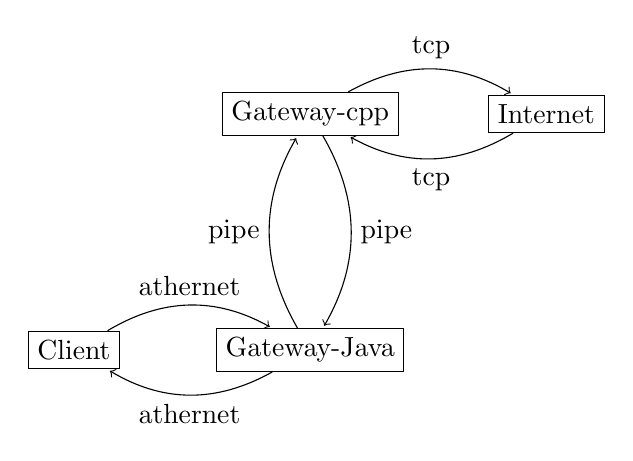
\begin{tikzpicture}[shorten >=1pt,node distance=3cm,on grid,auto]
		\node[rectangle, draw]	(q_0) 									{Client};
		\node[rectangle, draw] 	(q_1) 	[right=of q_0] 	{Gateway-Java};
		\node[rectangle, draw] 	(q_2) 	[above=of q_1] 	{Gateway-cpp};
		\node[rectangle, draw] 	(q_3) 	[right=of q_2] 	{Internet};
		\path[->]
			(q_0)		edge 	[bend left]			node 	{athernet} 	(q_1)
			(q_1) 	edge 	[bend left]			node 	{pipe} 	(q_2)
							edge 	[bend left]			node 	{athernet} 	(q_0)
			(q_2) 	edge 	[bend left]			node 	{pipe} 	(q_1)
							edge 	[bend left]			node 	{tcp} 	(q_3)
			(q_3) 	edge 	[bend left]			node 	{tcp} 	(q_2);
	\end{tikzpicture}

	%TOCHECK
	\subsection{JNI}
		The fact that there is no raw socket in Java requires us to use JNI to call c functions in Java.
		To use JNI, we have to write a wrapper in C that follows Java standard so that Java compiler can recognize it.
		We will not talk about the details here. 
		\par
		We found a company savarese() that open sourced it's JNI and all TCP related packet wrapper. 
		The work consists of two parts: the raw socket wrapper called Rocksaw(https://www.savarese.com/software/rocksaw/) and a TCP packet wrapper vserv(https://www.savarese.org/software/vserv-tcpip/).
		\par
		The major downfall of this method that directly lead us to bail is that raw socket requires root and that is not acceptable for a user application.
		Also, the tcp wrapper provided by savarese was nasty. 
		We reviewed the code to know the usage, that's when we found that the classes uses reference outside the object to do the job, which goes beyond the idea of the word "wrapper".
		\par
		As a result, we gave up Java. 
		We tried to do socket and TCP job using other languages and tries to communicate these two using some method.

	%TODO
	\subsection{Pipe}
		Finally we decided to use pipe for communication.
		One way pipe is relatively easy where you can type:
		\begin{center}\begin{lstlisting}
			program | another-program
		\end{lstlisting}\end{center}
		But to have a two way pipe is more difficult.
		It is hard because it's easy for two program get caught in dead lock where each one of them will not output anything until they are feed with some input. 
		Here we used Named Pipe which utilized file system to do the passing work.
		To use a named pipe, you have to do:
		\begin{lstlisting} 
			mkfifo fifo
			program1 <fifo | program 2 >fifo
		\end{lstlisting}
		\par
		In practice, both Java and C++ read from and output to stdin and stdout. 
		In this way, they can communicate with each other.

	%TODO: maybe nat_pack should be mentioned here? 
	\subsection{Nat Packet}
		Ernest please fill this part.
	
	%TOCHECK
	\subsection{Java experience: Cross platform}
		Before project 3 we did all the programming in Windows.
		The requirement of root privilege forced us to change to Ubuntu.
		However, we are happy to find that the code we wrote before can run directly with no problem on Ubuntu.
		The experience of Java's cross platform ability is somewhat refreshing.

	%TODO
	\subsection{C++ experience: Socket Programming}
		\paragraph{\textbf{gateway on the c++ side}}
		The c++ need to handle all Internet Communication and provide I/O service for the java gateway agent. In other words, the c++ gateway need to send out IP packets whenever the java gateway request sending, and give received packet from Internet to Java Interface (with some pre-pocessing).
		
		\paragraph{\textbf{TCP, UDP and ICMP}}
		For TCP and UDP, we are calling the interfaces provided by linux keneral interface, inlcuding \emph{socket}, \emph{binding}, \emph{connect}, \emph{sendto} and \emph{recefrom}. For ICMP, we are using the ICMP provided by Boost Libraries. 
		\paragraph{\textbf{TCP Receiving Buffer}}
		 One tricky part here is that TCP is streaming rather than transmitting packets, which results in that one frame may split into two frames when sending out. In order to solve the problem, for some application scenarioes, we use first several bytes to encode the length of the frame on sending and receiver store the current frame to buffer if it need to wait for the next frame.
		

%%%%%%%%%%%%%%%%%%%%%%%%%%%%%%%%%%%%%%%%%%%%%%%%%%%%%%%%%%%%%%%%%%%%%
%%
%% Project 4: FTP application
%%
%%%%%%%%%%%%%%%%%%%%%%%%%%%%%%%%%%%%%%%%%%%%%%%%%%%%%%%%%%%%%%%%%%%%%
\section{Project 4: FTP application}
	\subsection{Overview}	
	The FTP connection is handled mainly at the gateway side. The node A (athernet FTP client) is connected to node B through athernet. The node B (FTP gateway) is connected to FTP Server via Internet.
	\subsection{Passive Mode}
	For \emph{LIST} and \emph{RETR} command, passive mode need to be supported. The gateway parses every reply from FTP server before redirecting that to java client. Once the gateway received a reply starting with code 227, the reply from server with expected passive ports, the gateway records it as \emph{data\_port}. Then, if the gateway received a sending request of \emph{LIST} or \emph{RETR}, it immediately start a new TCP connection to the server with \emph{data\_port}.

%%%%%%%%%%%%%%%%%%%%%%%%%%%%%%%%%%%%%%%%%%%%%%%%%%%%%%%%%%%%%%%%%%%%%
%%
%% Course and Homework
%%
%%%%%%%%%%%%%%%%%%%%%%%%%%%%%%%%%%%%%%%%%%%%%%%%%%%%%%%%%%%%%%%%%%%%%
\section{Course}
	
	%TODO
	\subsection{Lectures}
	
	%TODO
	\subsection{Homework}

	%TODO
	\subsection{Projects}

%%%%%%%%%%%%%%%%%%%%%%%%%%%%%%%%%%%%%%%%%%%%%%%%%%%%%%%%%%%%%%%%%%%%%
%%
%% Acknowledgement
%%
%%%%%%%%%%%%%%%%%%%%%%%%%%%%%%%%%%%%%%%%%%%%%%%%%%%%%%%%%%%%%%%%%%%%%
%TOCHECK
\section*{Acknowledgment}
	Finally, we would like to thank Zhice for providing us with such a great course.
	The projects you prepared is really exciting and challenging. 
	We learned a lot during this course.
	We would like thank Fengling and Cheng too. 
	They spend 4 weekends to check out project and patiently waited for us until late.
	Thanks for the effort.
	Finally we would like to thank Anqi, who provided a lot of ideas to us.

\bibliographystyle{IEEEtran}
\bibliography{report}


% that's all folks
\end{document}


